\ifdefined\activerhandout 
\documentclass[12pt,aspectratio=1610,handout]{beamer}
\else
\documentclass[12pt,aspectratio=1610]{beamer}
\fi

%\usepackage[french]{babel} %=> erreur avec les tikz du moteur
\usepackage[T1]{fontenc}
\usepackage[utf8]{inputenc}
\usepackage{lmodern}
\usepackage{hyperref}
\usepackage{smartdiagram}
\usepackage{tikz}
\usepackage{animate}
\usepackage{tikzpeople}
\usepackage{appendixnumberbeamer}
\usepackage[labelformat=empty]{caption}
%\usepackage{pictochrono}
\usepackage{fontawesome5}
\usepackage{awesomebox}

\usetheme{Warsaw}
\setbeamertemplate{page number in head/foot}[totalframenumber]

\newcommand{\anglais}[1]{(\textit{\color{blue}#1})}
\newcommand{\legende}[2]{\caption[#1 (Source : \cite{#2})]{#1}}
\newcommand{\histoire}[1]{\begin{awesomeblock}{2pt}{\faBook}{black!75}#1\end{awesomeblock}}
\newcommand{\info}[1]{\begin{awesomeblock}{2pt}{\faInfoCircle}{black!75}#1\end{awesomeblock}}
\newcommand{\question}[1]{\begin{awesomeblock}{2pt}{\faQuestionCircle}{black!75}#1\end{awesomeblock}}
\newcommand{\alerte}[1]{\begin{awesomeblock}{2pt}{\faExclamationCircle}{black!75}#1\end{awesomeblock}}
\newcommand{\astuce}[1]{\begin{awesomeblock}{2pt}{\faLightbulb}{black!75}#1\end{awesomeblock}}
\newcommand{\exemple}[1]{\begin{awesomeblock}{2pt}{\faSearch}{black!75}#1\end{awesomeblock}}
\newcommand{\definitionAConnaitre}[1]{\begin{awesomeblock}{2pt}{\faCog}{black!75}#1\end{awesomeblock}}

\newcommand{\qmcBia}[7]{
%1 : titre slide
%2 : numéro de la bonne réponse
%3 : Inititulé de la question
%4, 5, 6, et 7 : propositions de réponse
\begin{frame}{#1}
\begin{awesomeblock}{2pt}{\faQuestion}{black!75}
#3
	\begin{enumerate}
	\ifnum#2=1
		\only<1>{\item #4}
		\only<2>{\item \textbf{#4}}
	\else
		\item #4
	\fi
	\ifnum#2=2
		\only<1>{\item #5}
		\only<2>{\item \textbf{#5}}
	\else
		\item #5
	\fi
	\ifnum#2=3
		\only<1>{\item #6}
		\only<2>{\item \textbf{#6}}
	\else
		\item #6
	\fi
	\ifnum#2=4
		\only<1>{\item #7}
		\only<2>{\item \textbf{#7}}
	\else
		\item #7
	\fi
	\end{enumerate}
	\pause
\end{awesomeblock}
\end{frame}
}

\subtitle{BIA - Brevet d'Initiation Aéronautique}
\author{Clément \textsc{Vermot-Desroches}}
\institute{Collège Aliénor d'Aquitaine\\Martignas-sur-Jalle}
\date{\today}

%\AtBeginSection[]
%{
%    \begin{frame}
%        %\frametitle{Table of Contents}
%        \tableofcontents[currentsection]
%    \end{frame}
%}

\AtBeginSubsection[]
{
    \begin{frame}
        %\frametitle{Table of Contents}
        \tableofcontents[currentsection,currentsubsection]
    \end{frame}
}
% Author: Izaak Neutelings (November 2020)
%\documentclass[border=3pt,tikz]{standalone}
%\usepackage{siunitx}
%\usepackage{physics}
%\usepackage{tikz}
%\usepackage[outline]{contour} % glow around text

%\begin{document}

\usetikzlibrary{patterns,decorations.pathmorphing}
\usetikzlibrary{arrows.meta}
\tikzset{>=latex}
\contourlength{1.1pt}

\colorlet{mydarkblue}{blue!50!black}
\colorlet{myred}{red!65!black}
\colorlet{watercol}{blue!80!cyan!10!white}
\colorlet{darkwatercol}{blue!80!cyan!20!white}
\tikzstyle{piston}=[blue!50!black,top color=blue!30,bottom color=blue!50,middle color=blue!20,shading angle=0]
\tikzstyle{water}=[draw=mydarkblue,top color=watercol!90,bottom color=watercol!90!black,shading angle=5]
\tikzstyle{vertical water}=[water,
  top color=watercol!90!black!90,bottom color=watercol!90!black!90,middle color=watercol!80,shading angle=90]
\def\tick#1#2{\draw[thick] (#1)++(#2:0.1) --++ (#2-180:0.2)}

\def\barometreTorricelli#1{
%parametre 1 : hauteur en mm de mercure => mmHg
% PRESSURE TORRICELLI

  %\def\mmHg{760}
  \def\mmHg{#1}
  \def\Rx{1.8}
  \def\Ry{0.05}
  \def\rx{0.18}
  \def\ry{0.06*\rx/1.5}
  \def\H{1.0}
  \def\h{0.72*\H}   % water level height
  \def\th{3.2*\H}   % tube height
  \def\ty{\mmHg/1000*\th} % tube level
  \def\td{0.6*\h}   % tube depth
  \def\N{10}
  
  % WATER + CONTAINER
  \draw[vertical water] %rounded corners=2
    (-\Rx,\h) --++ (0,-\h) arc(180:360:{\Rx} and {\Ry}) --++ (0,\h);
  \draw[water]
    (0,\h) ellipse ({\Rx} and {\Ry});
  \draw[thick] (0,\H) ellipse ({\Rx} and {\Ry});
  
  % TUBE
  \draw[vertical water]
    (-\rx,\h) |-++ (2*\rx,\ty) --++ (0,-\ty);
  \draw[water]
    (0,\h+\ty) ellipse ({\rx} and {\ry});
  \draw[thick,line cap=round]
    (-\rx,\h) --++ (0,\th) coordinate (T) arc(180:0:\rx) --++ (0,-\th);
  \draw[mydarkblue,line cap=round]
    (-1.09*\rx,\h-0.005) arc(180:360:{1.09*\rx} and 1.12*\ry);
  \foreach \i [evaluate={\y=1.12*\H+0.84*\th*\i/\N}] in {0,...,\N}{
    \draw[line cap=round] (\rx,\y) arc(0:-50:{\rx} and \ry);
  }
  \begin{scope}
    \clip (-\Rx,\h) |-++ (2*\Rx,-\h) --++ (0,\h) arc(360:180:{\Rx} and {\Ry}) -- cycle;
    \draw[thick,line cap=round]
      (-\rx,\h) --++ (0,-\td) (\rx,\h) --++ (0,-\td);
      %(-\rx,\h) --++ (0,-\td) arc(180:360:{\rx} and {\ry}) --++ (0,\td);
    \draw[vertical water,opacity=0.5]
      (-\Rx,\h) --++ (0,-\h) arc(180:360:{\Rx} and {\Ry}) --++ (0,\h);
  \end{scope}
  \draw[mydarkblue]
    (-\Rx,\h) arc(180:360:{\Rx} and {\Ry});
  \draw[<->] (0.8*\Rx,\h) --++ (0,\ty) node[midway,fill=white,inner sep=1] {$h =\pgfmathparse{\mmHg}\pgfmathprintnumber{\pgfmathresult}~mm$};
  \draw[very thin,line cap=round]
    (T)++(130:\rx) node[anchor=-19,inner sep=1] {$Vide$} to[out=-50,in=170]++ (-30:1.5*\rx);
  \node[above] at (-0.6*\Rx,\H) {$P_\mathrm{atm}$};
  
  % CONTAINER
  \draw[thick]
    (-\Rx,\H) --++ (0,-\H) arc(180:360:{\Rx} and {\Ry})
              --++ (0,\H) arc(360:180:{\Rx} and {\Ry}) -- cycle;
              
  }
	


	
%\end{document}
%\documentclass[tikz,border=6pt]{standalone}
%\usepackage{tikz}
\usetikzlibrary{calc,backgrounds}
%\usepackage{ifthen}

%\begin{document}

\pgfdeclareimage{montagne}{commun/img/montagne.pdf}

\newcommand{\echelleAltitudeMetres}[2]{
%\begin{tikzpicture}[x=1cm,y=1cm, scale=0.6, every node/.style={scale=0.6}] % 1 unité = 1 km = 1000 m

% --------- paramètres (modifiables) ----------
\def\maxkm{#1}            % hauteur totale en km (10 = 10000 m)
\def\pointeralt{#2}      % position curseur en km (5 = 5000 m)
\def\pointerside{right}   % 'left' ou 'right' (placement du curseur)
% limites horizontales de la montagne (choisis des valeurs <= -1.6 pour ne pas empiéter sur l'axe)
\def\positionMontagne{-4.9}      % bord gauche de la base
% ---------------------------------------------

% configuration curseur selon côté
\ifthenelse{\equal{\pointerside}{right}}{%
  \def\pointerx{0.45}%
  \def\labelanchor{west}%
  \def\xshift{6pt}%
}{%
  \def\pointerx{-0.45}%
  \def\labelanchor{east}%
  \def\xshift{-6pt}%
}

% cadre optionnel pour cadrer
	\draw[gray!0] (\positionMontagne,0) rectangle (2.5,\maxkm+0.3);

% Axe vertical (altitude)
\draw[line width=0.6pt] (0,0) -- (0,\maxkm+0.3);
% graduations 1000 m (1 km)
\foreach \k in {0,...,10}{
  \pgfmathtruncatemacro{\lab}{\k*1000}
  \draw (-0.12,\k) -- (0.12,\k);
  \node[left=3pt] at (-0.15,\k) {\small \lab\ m};
}
% étiquette d'axe "Altitude" déplacée plus à gauche pour ne pas être masquée
\node[rotate=90] at (-2.0,\maxkm/2) {\large Altitude};

\node at (\positionMontagne,0) {\pgfbox[0,0]{\pgfuseimage{montagne}}};

% --- Curseur triangulaire bleu sur le côté choisi (par défaut à droite) ---
\begin{scope}
  \fill[blue!70!black] (0,\pointeralt) -- (\pointerx,\pointeralt+0.22) -- (\pointerx,\pointeralt-0.22) -- cycle;
  \draw[blue!90!black,line width=0.6pt] (0,\pointeralt) -- (\pointerx,\pointeralt+0.22) -- (\pointerx,\pointeralt-0.22) -- cycle;
  \pgfmathtruncatemacro{\pointerm}{\pointeralt*1000}
  \node[anchor=\labelanchor, xshift=\xshift] at (\pointerx,\pointeralt) {\small \pointerm\ m};
\end{scope} 
}


%\end{tikzpicture}
%\end{document}


\title[Séance 5 - Atmosphère]{Séance 5 \\ Atmosphère}

\begin{document}
 \begin{frame}
 \titlepage
 \end{frame}
 
 \begin{frame}
 \tableofcontents
 \end{frame}
 
 \section{L'atmosphère}
	\begin{frame}{L'atmosphère}
	
	\question{Qu'est-ce que l'atmosphère ?}
	\pause
	\question{De quoi est composée l'atmosphère ?}
	\end{frame}	 
	
	\begin{frame}{La composition de l'atmosphère terrestre}
	L'air sec est composé de :
	\begin{table}[H]
	\begin{tabular}{|l|c|}
		\hline
		Gaz & Proportion \\
		\hline
		\hline
		Azote ($N$) & 78~\% \\
		\hline
		Oxygène ($O$) & 21~\% \\
		\hline
		Argon ($Ar$) & 0,9~\% \\
		\hline
		Autres gaz (dont Dioxyde de carbone ($CO_2$)) & 0,1~\% \\
		\hline
	\end{tabular}
	\caption{Composition de l'atmosphère terrestre}
	\end{table}
	\end{frame}

 	\begin{frame}{Les couches de l'atmosphère terrestre}
 		\begin{columns}
 		\begin{column}{0.4\textwidth}
		\begin{figure}[H]
			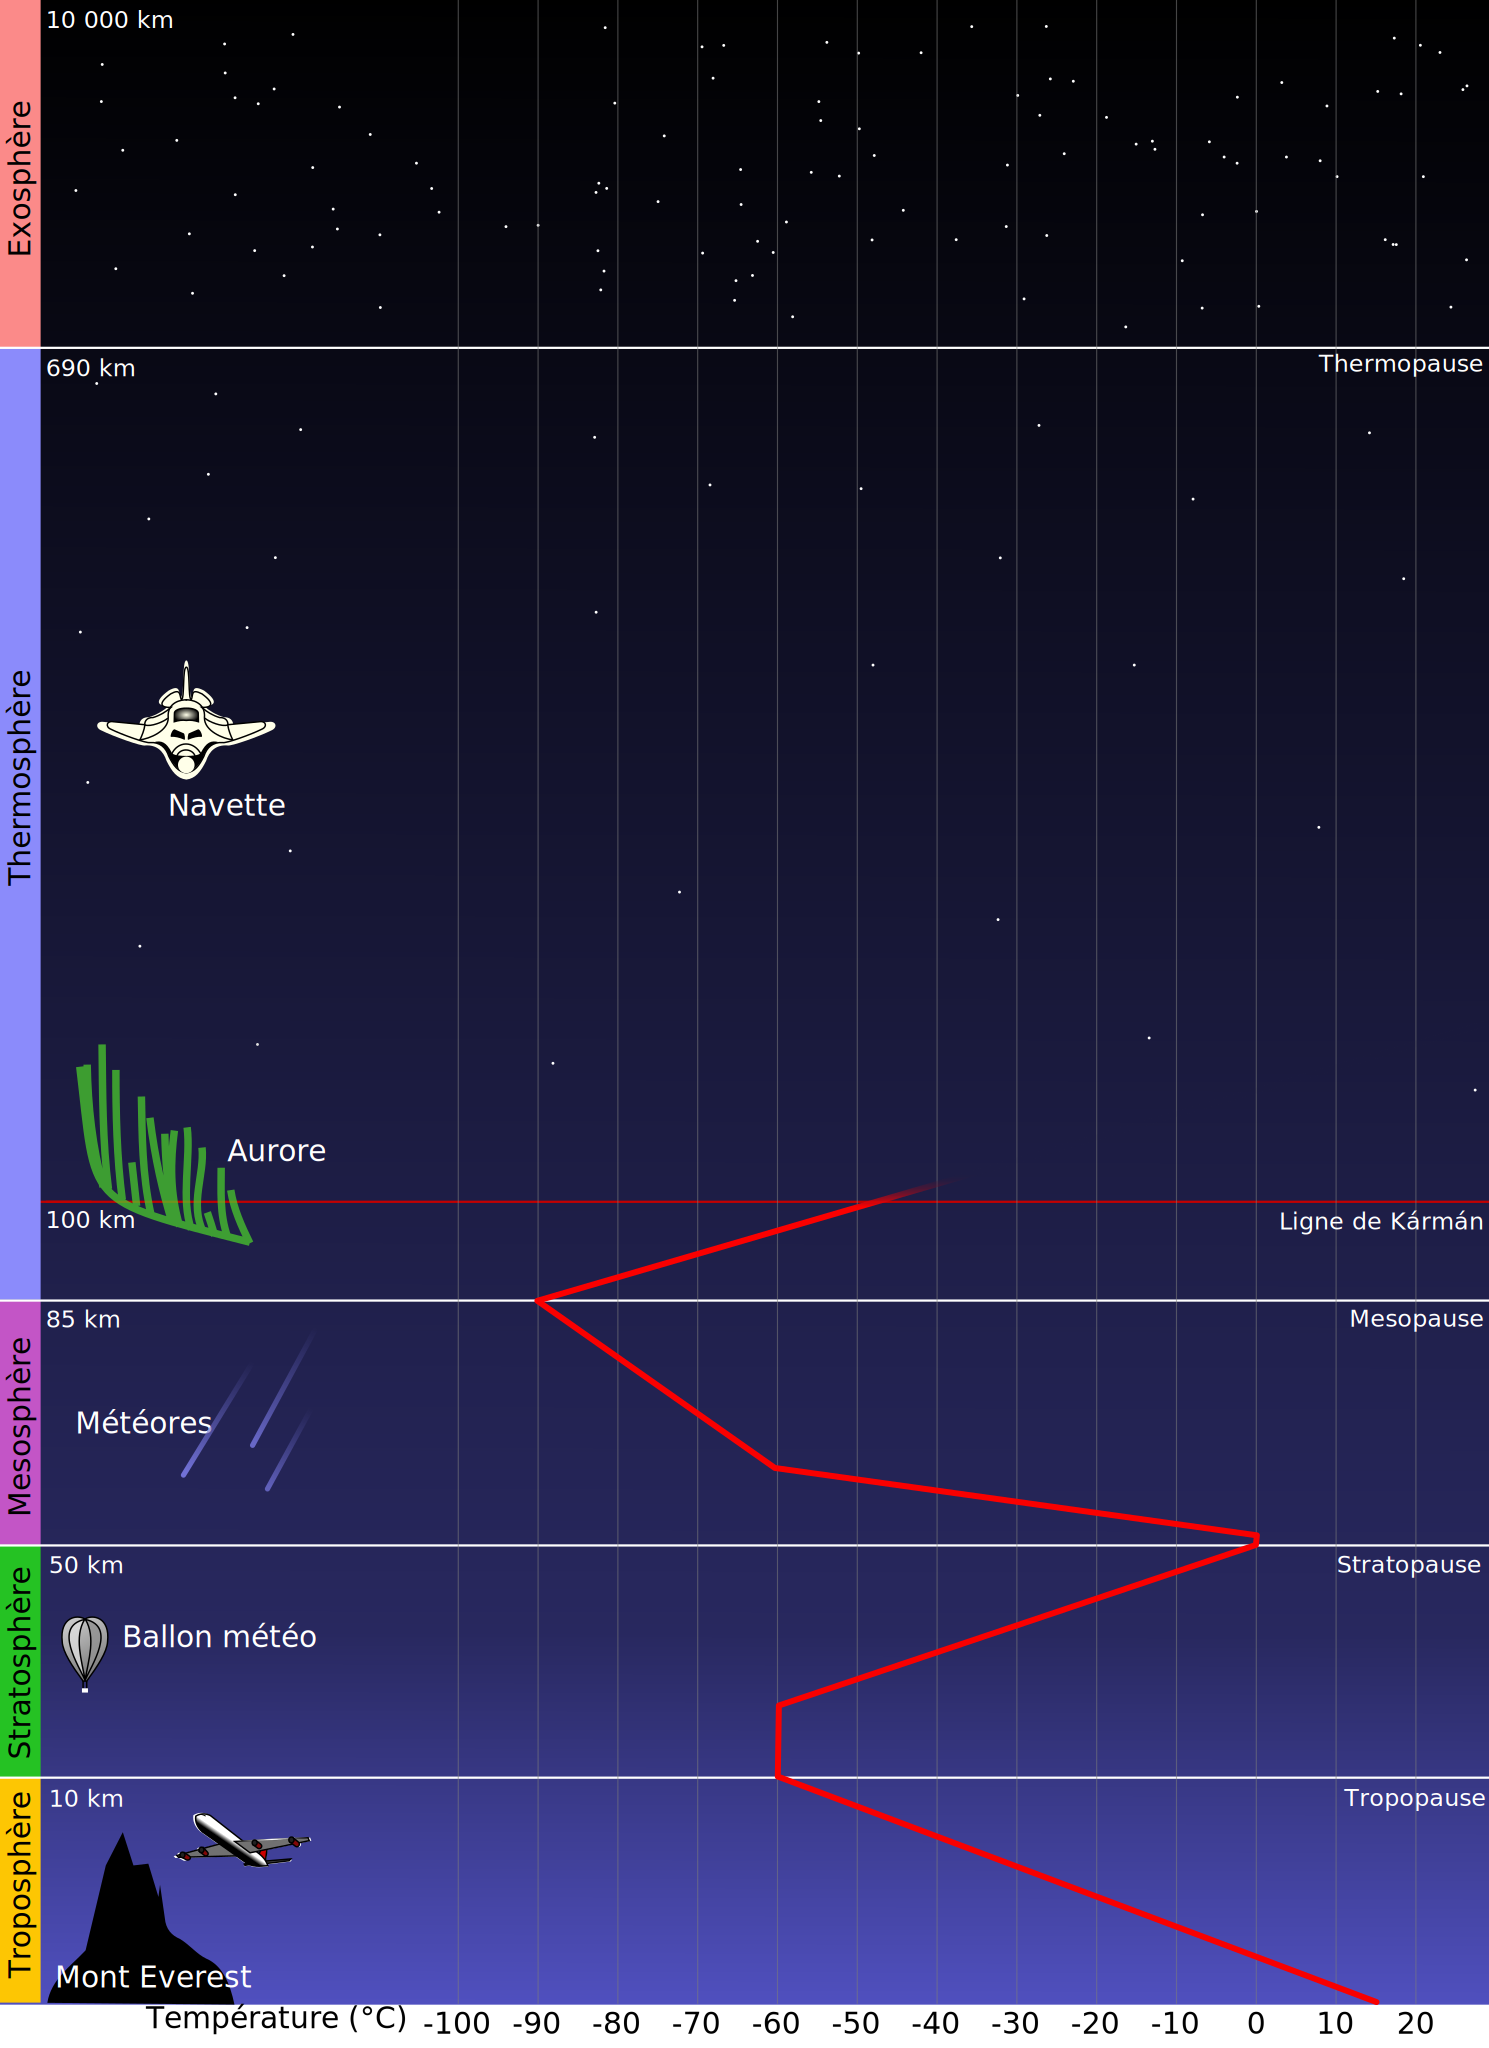
\includegraphics[width=0.95\linewidth]{03-Meteo/img/couchesAtmosphereTemperature.pdf}
			\legende{Schéma des couches de l'atmosphère}{img:couchesAtmosphereTemperature}
			\end{figure}	
		\end{column}
 		\begin{column}{0.6\textwidth}
 			On s'intéressera surtout à la troposphère, zone ou évoluent les aéronefs et ou se déroulent l'essentiel des phénomènes climatiques.
 		\end{column}
 		\end{columns}
	\end{frame}	
	
	\begin{frame}{La pression atmosphérique}
	Tout l'air au dessus de nous est soumis à la gravité terrestre. Il a donc un poids.
	
	\begin{figure}
	\begin{tikzpicture}
	\barometreTorricelli{760} 
	\end{tikzpicture}
	\legende{Baromètre de Torricelli au mercure, au niveau de la mer}{img:barometreTorricelli}
	\end{figure}
	\end{frame}
	
	\begin{frame}{La pression atmosphérique et l'altitude}
	\begin{figure}[H]
		\ifdefined\activeranimations 
		\newcommand{\nbFramesAltitude}{101}
		\else
		\newcommand{\nbFramesAltitude}{1}
		\fi
		
		%760 mmHg à 0 m
		%200 mmHg à 10 000 m
		%=> 560 mmHg entre les 2, soit, pour 100 frames, 5.6
		%\newcommand{\altToMmHg}{((760-200)/\nbFramesAltitude)}
		%\newcommand{\altToMmHg}{0.2}
		
		\centering
		\begin{animateinline}[controls,loop]{8}
		    \multiframe{\nbFramesAltitude}{i=0+1}{
			\begin{tikzpicture}[x=1cm,y=1cm, scale=0.7, every node/.style={scale=0.7}]
				\echelleAltitudeMetres{10}{\i/10}
			\end{tikzpicture}
			\begin{tikzpicture}[scale=1.5, every node/.style={scale=1.5}]
				%\FPeval{\asoustraire}{clip(\i*\altToMmHg)}
				\FPeval{\result}{round((760-\i*5.6),0)}
				\barometreTorricelli{\result}		
			\end{tikzpicture}
			}
		\end{animateinline}
	\end{figure}
	\end{frame}
	
	\begin{frame}{L'atmosphère standard}
			On fixe les caractéristiques d'une atmosphère dite "standard" (ISA) comme suit :
			\begin{itemize}
				\item Température au niveau de la mer : $\ang{15}C$
				\item Pression atmosphérique au niveau de la mer : $1013,25~hPa$
			\end{itemize}
			
			Dans cette atmosphère standard, ces grandeurs évoluent comme ceci :
			\begin{itemize}
				\item $\ang{-0.65}C$ tous les $100~m$ (soit $\ang{-2}C$ tous les $1000~ft$), jusqu'à la tropopause
				\item $-1~hPa$ tous les $8,5~m$ (soit $-1~hPa$ tous les $28~ft$)
			\end{itemize}
	\end{frame}
	
	\begin{frame}{La pression atmosphérique à l'échelle d'un continent}
	\begin{columns}
 		\begin{column}{0.6\textwidth}
		\begin{figure}[H]
			\includegraphics[width=1\linewidth]{03-Meteo/img/frontIsobares20260127.png}
			\legende{Carte des isobares}{img:frontIsobares20260127}
		\end{figure}	
		\end{column}
		\begin{column}{0.4\textwidth}
			Cette carte présente les lignes d'égales pression (isobares) \\
			
			Les zones notées $D$ sont des zones de faible pression : les \textbf{dépressions}
			
			Les zones notées $A$ sont des zones de hautes pression : les \textbf{anticyclones} \\
			
			Plus les lignes isobares sont rapprochées, plus le vent est fort.
		\end{column}
		\end{columns}
	\end{frame}
	
	\begin{frame}{Le vent}
		La loi de Buys-Ballot indique que quand on est face au vent, l'anticyclone est à gauche, et la dépression à droite, dans l'hémisphère nord (l'inverse dans l'hémisphère sud).
		\begin{figure}[H]
			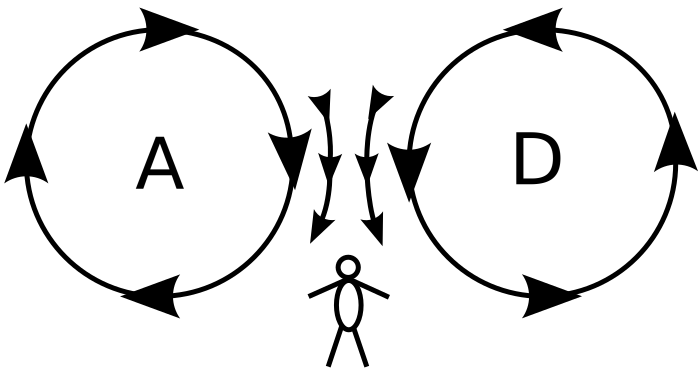
\includegraphics[width=0.4\linewidth]{03-Meteo/img/buysBallot.pdf}
			\legende{Illustration de la loi de Buys-Ballot}{img:buysBallot}
		\end{figure}	
		
		\astuce{Pour s'en souvenir, dans l'hémisphère nord (le notre) : les A : f\textbf{a}ce au vent, \textbf{a}nticyclone à g\textbf{a}uche.}
		
	\end{frame}
	
	\section{Les fronts}
	\begin{frame}{Les fronts}
	
		\begin{columns}
		\begin{column}{0.4\textwidth}
		Les masses d'air de l'atmosphère se différencient par leur température.
		
		La différence de température entre 2 masses d'air va provoquer, lors de leurs mouvements, le déplacement relatif sur le plan vertical des masses d'air.
		
		L'air chaud, plus léger, aura tendance à se soulever.
		\end{column}
		\begin{column}{0.6\textwidth}
		\begin{figure}[H]
			\includegraphics[width=1\linewidth]{03-Meteo/img/temsiEuroc20260127.png}
			\legende{Carte TEMSI}{img:temsiEuroc20260127}
		\end{figure}	
		\end{column}
		\end{columns}
	
	\end{frame}
	
	\begin{frame}{Front froid~~~~\includegraphics[width=0.3\linewidth]{03-Meteo/img/legendeFrontFroid.pdf}}
		\begin{figure}[H]
			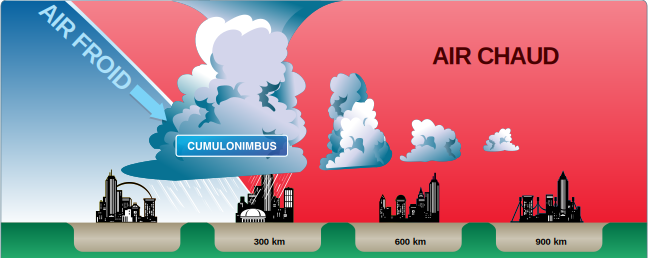
\includegraphics[width=1\linewidth]{03-Meteo/img/frontFroid.pdf}
			\legende{Coupe d'un front froid}{img:frontFroid}
		\end{figure}	
	\end{frame}

	\begin{frame}{Front chaud~~~~\includegraphics[width=0.3\linewidth]{03-Meteo/img/legendeFrontChaud.pdf}}
		\begin{figure}[H]
			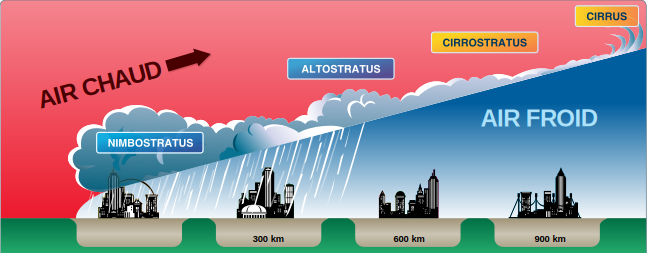
\includegraphics[width=1\linewidth]{03-Meteo/img/frontChaud.pdf}
			\legende{Coupe d'un front chaud}{img:frontChaud}
		\end{figure}	
	\end{frame}
	
	\begin{frame}{Front occlus~~~~\includegraphics[width=0.3\linewidth]{03-Meteo/img/legendeFrontOcclus.pdf}}
		\begin{figure}[H]
			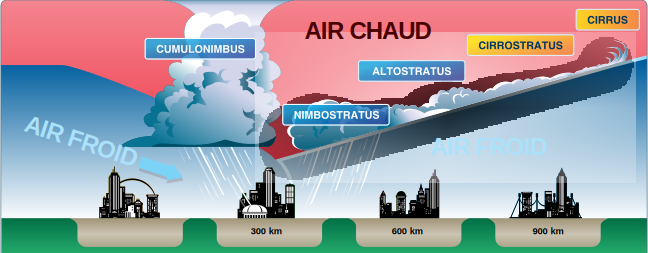
\includegraphics[width=1\linewidth]{03-Meteo/img/frontOcclus.pdf}
			\legende{Coupe d'un front occlus}{img:frontOcclus}
		\end{figure}	
	\end{frame}
 
\appendix 
\section{QCM}
\qmcBia{Météo}
{1}{Les deux principaux composants de l'air sec sont :}
{le diazote et le dioxygène}
{l'oxygène et le gaz carbonique}
{l'azote et l'hélium}
{l'oxygène et l'hydrogène} 
{}

\qmcBia{Météo}
{4}{La transformation de l'eau de l'état gazeux à l'état liquide s'appelle :}
{la fusion}
{la sublimation}
{l'évaporation}
{la condensation} 
{fusion = solide (glace) vers liquide \\ évaporation = liquide vers gazeux \\ sublimation = \pause solide (glace) vers gazeux }

\qmcBia{Météo}
{2}{Sur une carte de pression une ligne qui joint les points d'égale pression est nommée :}
{une isotherme}
{une isobare}
{une isocline}
{une isophypse} 
{isotherme = lignes d'égales température \\ isocline = ligne d'égale inclinaison magnétique \\ isophypse = ligne d'égale altitude}

\qmcBia{Météo}
{1}{Un front froid :}
{est une surface séparant un air froid en mouvement d'un air plus chaud qu'il soulève}
{est l'arrivée d'un air froid sur une surface polaire glacée}
{est l'arrivée d'un air froid et lourd qui stabilise la basse couche atmosphérique}
{est généralement associé à des brises marines d'ouest} 
{}

\qmcBia{Météo}
{2}{La couche de l'atmosphère où se concentrent les phénomènes météorologiques est la :}
{stratosphère}
{troposphère}
{mésosphère}
{thermosphère} 
{}

\qmcBia{Météo}
{4}{Une information sur une carte stipule l'ISO 0°C au FL80. Vous devez voler au FL60. En considérant le gradient standard, quelle est la bonne affirmation ?}
{Le vol se fera à +4 °C}
{Le vol se fera à -4 °C}
{Le vol se fera à -2 °C}
{Le vol se fera à +2 °C} 
{FL80 = 8000 pieds, FL60 = 6000 pieds \\ On vole 2000 pieds sous l'isotherme 0°, et on sait que l'on perd 2° par 1000 pieds, donc on sera 4°C plus chaud qu'au FL80}

 
\ifdefined\activerbibliobeamer
\begin{frame}[allowframebreaks]
\frametitle{Bibliographie}
\printbibliography
%\nocite{*}
\end{frame}
\fi 
 
\end{document}
